%%%%%%
%
% $Autor: Sudeshna Nanda $
% $Datum: 2024-10-19 $
% $Pfad: ML23-06-Magic-Wand-with-an-Arduino-Nano-33-BLE-sense/manual/Contents/en/ProductMainFunctions.tex $
% $Version: 1 $
%
%%%%%%



\chapter{Product Main Functions}

\section{Switching On}\label{switching on}
Connect the Cable Micro USB here for power inlet, The Power LED indicates whether the main power is connected. The light will turn to green once you connect.

\section{Motion Movement}\label{Motion Movement}
Your Magic Wand is equipped with a state-of-the-art motion sensor capable of detecting a wide range of movements. Each gesture corresponds to a magical command that activates different light colors.

\subsection{Wings}
Hold your arm straight out in front of you with the wand pointing up. Start by moving the wand down toward your lower right, then bring it up to the middle, creating the first “V” shape. From the middle, move the wand down again toward your lower left, and then back up to the upper right, completing the second “V” shape. Together, these motions form a "W" shape in the air. The figure below shows the direction of the movements. A red color generates when the wing gesture is recognized.

\begin{figure}[h]
	\centering
	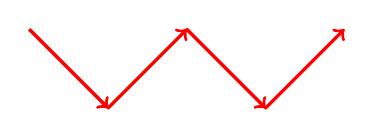
\begin{tikzpicture}
		% Define points
		\coordinate (A)  at (1, 1);
		\coordinate (O)  at (2, 0);
		\coordinate (B)  at (3, 1);
		\coordinate (C)  at (4, 0);
		\coordinate (D)  at (5, 1);
		
		% Draw the W shape
		\draw[thick, red] (A) -- (O) -- (B) -- (C) -- (D);
		
		% Draw arrows for direction
		\draw[->, very thick, red] (1,1) -- (2,0)  node [midway, above] {};
		\draw[->, very thick, red] (2,0) -- (3,1)  node [midway, above] {};
		\draw[->, very thick, red] (3,1) -- (4,0)  node [midway, above] {};
		\draw[->, very thick, red] (4,0) -- (5,1)  node [midway, above] {};
	\end{tikzpicture}
	\caption{\textbf{Wing Gesture}}
	\label{fig:Wing_Gesture}
\end{figure}

\subsection{Rings}
Hold the wand vertically in front of you. Move the wand in a circular motion, drawing a ring in the air. Ensure the motion is smooth and steady, completing the circle. A green color generates when the ring gesture is detected.

\begin{figure}[h]
	\centering
	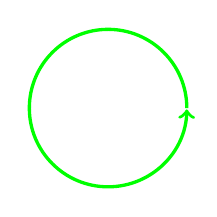
\begin{tikzpicture}
		\draw[->,very thick,green] (0,0) arc[radius=1cm,start angle=0,delta angle=359];
	\end{tikzpicture}
	\caption{\textbf{Ring Gesture}}
	\label{fig:Ring_Gesture}
\end{figure}

\subsection{Slope}
Point the wand up and hold your arm straight out in front of you. Start by moving the wand in a downward slope from the higher right to the lower left. Complete the shape by extending the wand horizontally to the left, creating a diagonal line in the air. A blue color generates when the slope gesture is detected.

\begin{figure}[h]
	\centering
	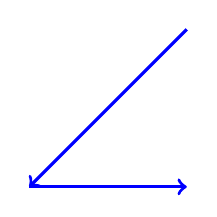
\begin{tikzpicture}
		% Define points
		\coordinate (A) at (2, 2);
		\coordinate (O) at (0, 0);
		\coordinate (B) at (2, 0);
		
		% Draw lines for slope
		\draw[->, very thick, blue] (2,2) -- (0,0) node[midway, above] {};
		\draw[->, very thick, blue] (0,0) -- (2,0) node[midway, above] {};
	\end{tikzpicture}
	\caption{\textbf{Slope Gesture}}
	\label{fig:Slope_Gesture}
\end{figure}

\subsection{Unknown}

All gesture movements apart from the three types mentioned above will appear as a cross shape in the monitor output. A yellow light generates when unknown gestures are discovered.

\begin{figure}[h]
	\centering
	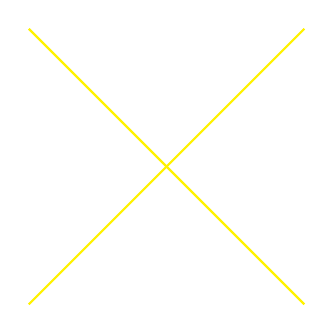
\begin{tikzpicture}
		% Draw cross shape in yellow
		\draw[thick, yellow] (-2, 2.5) -- (1.5, -1);
		\draw[thick, yellow] (1.5, 2.5) -- (-2, -1);
	\end{tikzpicture}
	\caption{\textbf{Unknown Output}}
	\label{fig:Unknown_Gesture}
\end{figure}



\section{Reset Magic Wand}\label{Reset Magic Wand}
Press the reset button once on the board if the magic wand does not run properly. You will see all the led lights would fade out at once and the Power LED will fade in back after clicking. This can help to run the program from the beginning.

%\begin{figure}[h!]
%	\centering	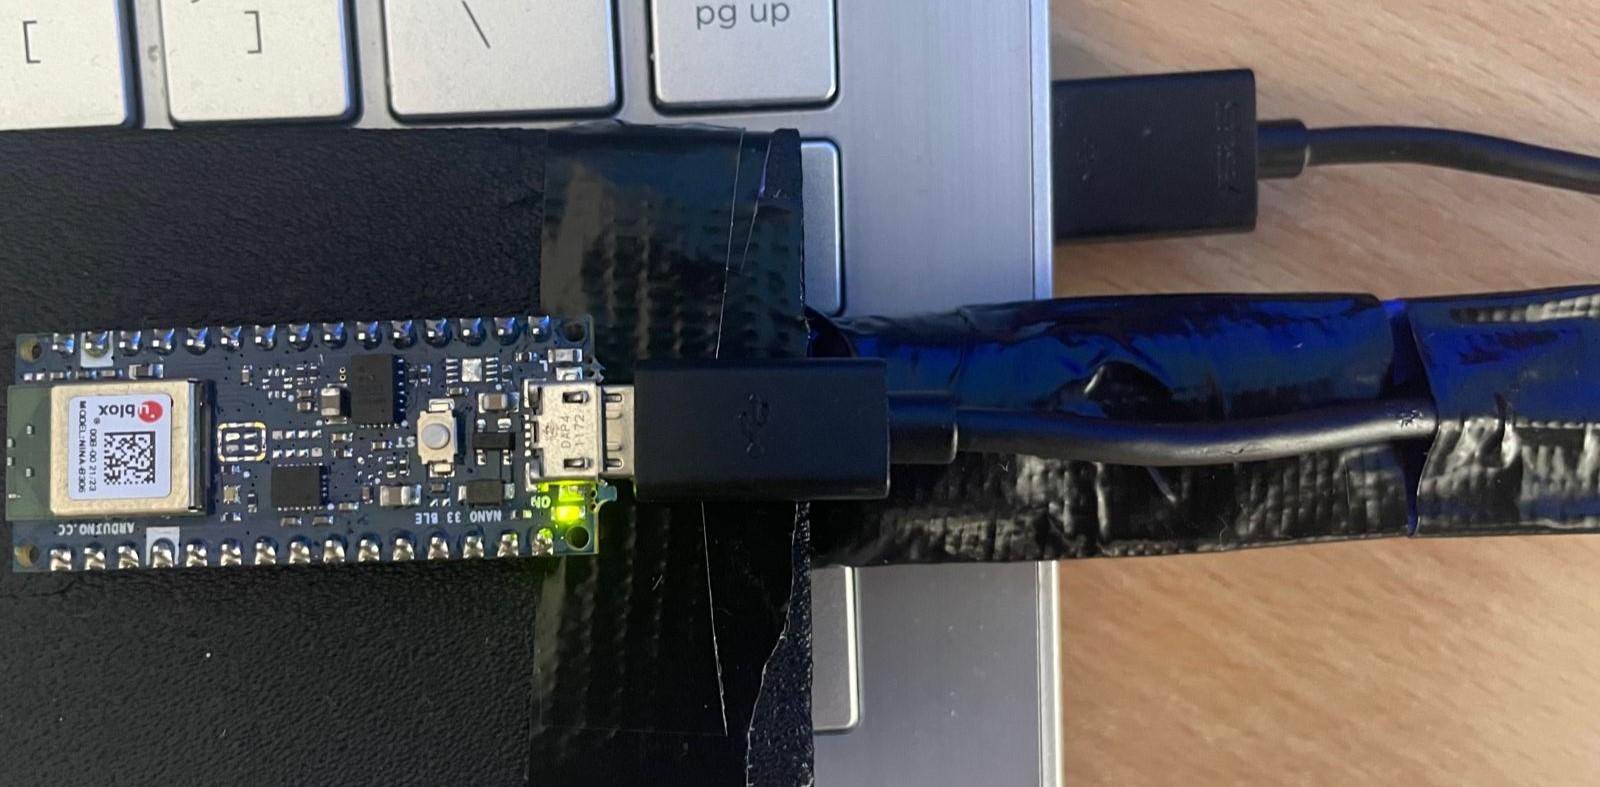
\includegraphics[width=15cm]{Images/usbb}
%	\caption{\textbf{How to connect with computer}}
%\end{figure}

%\section{Connector Pinouts}
%\begin{figure}[h!]
	%\centering	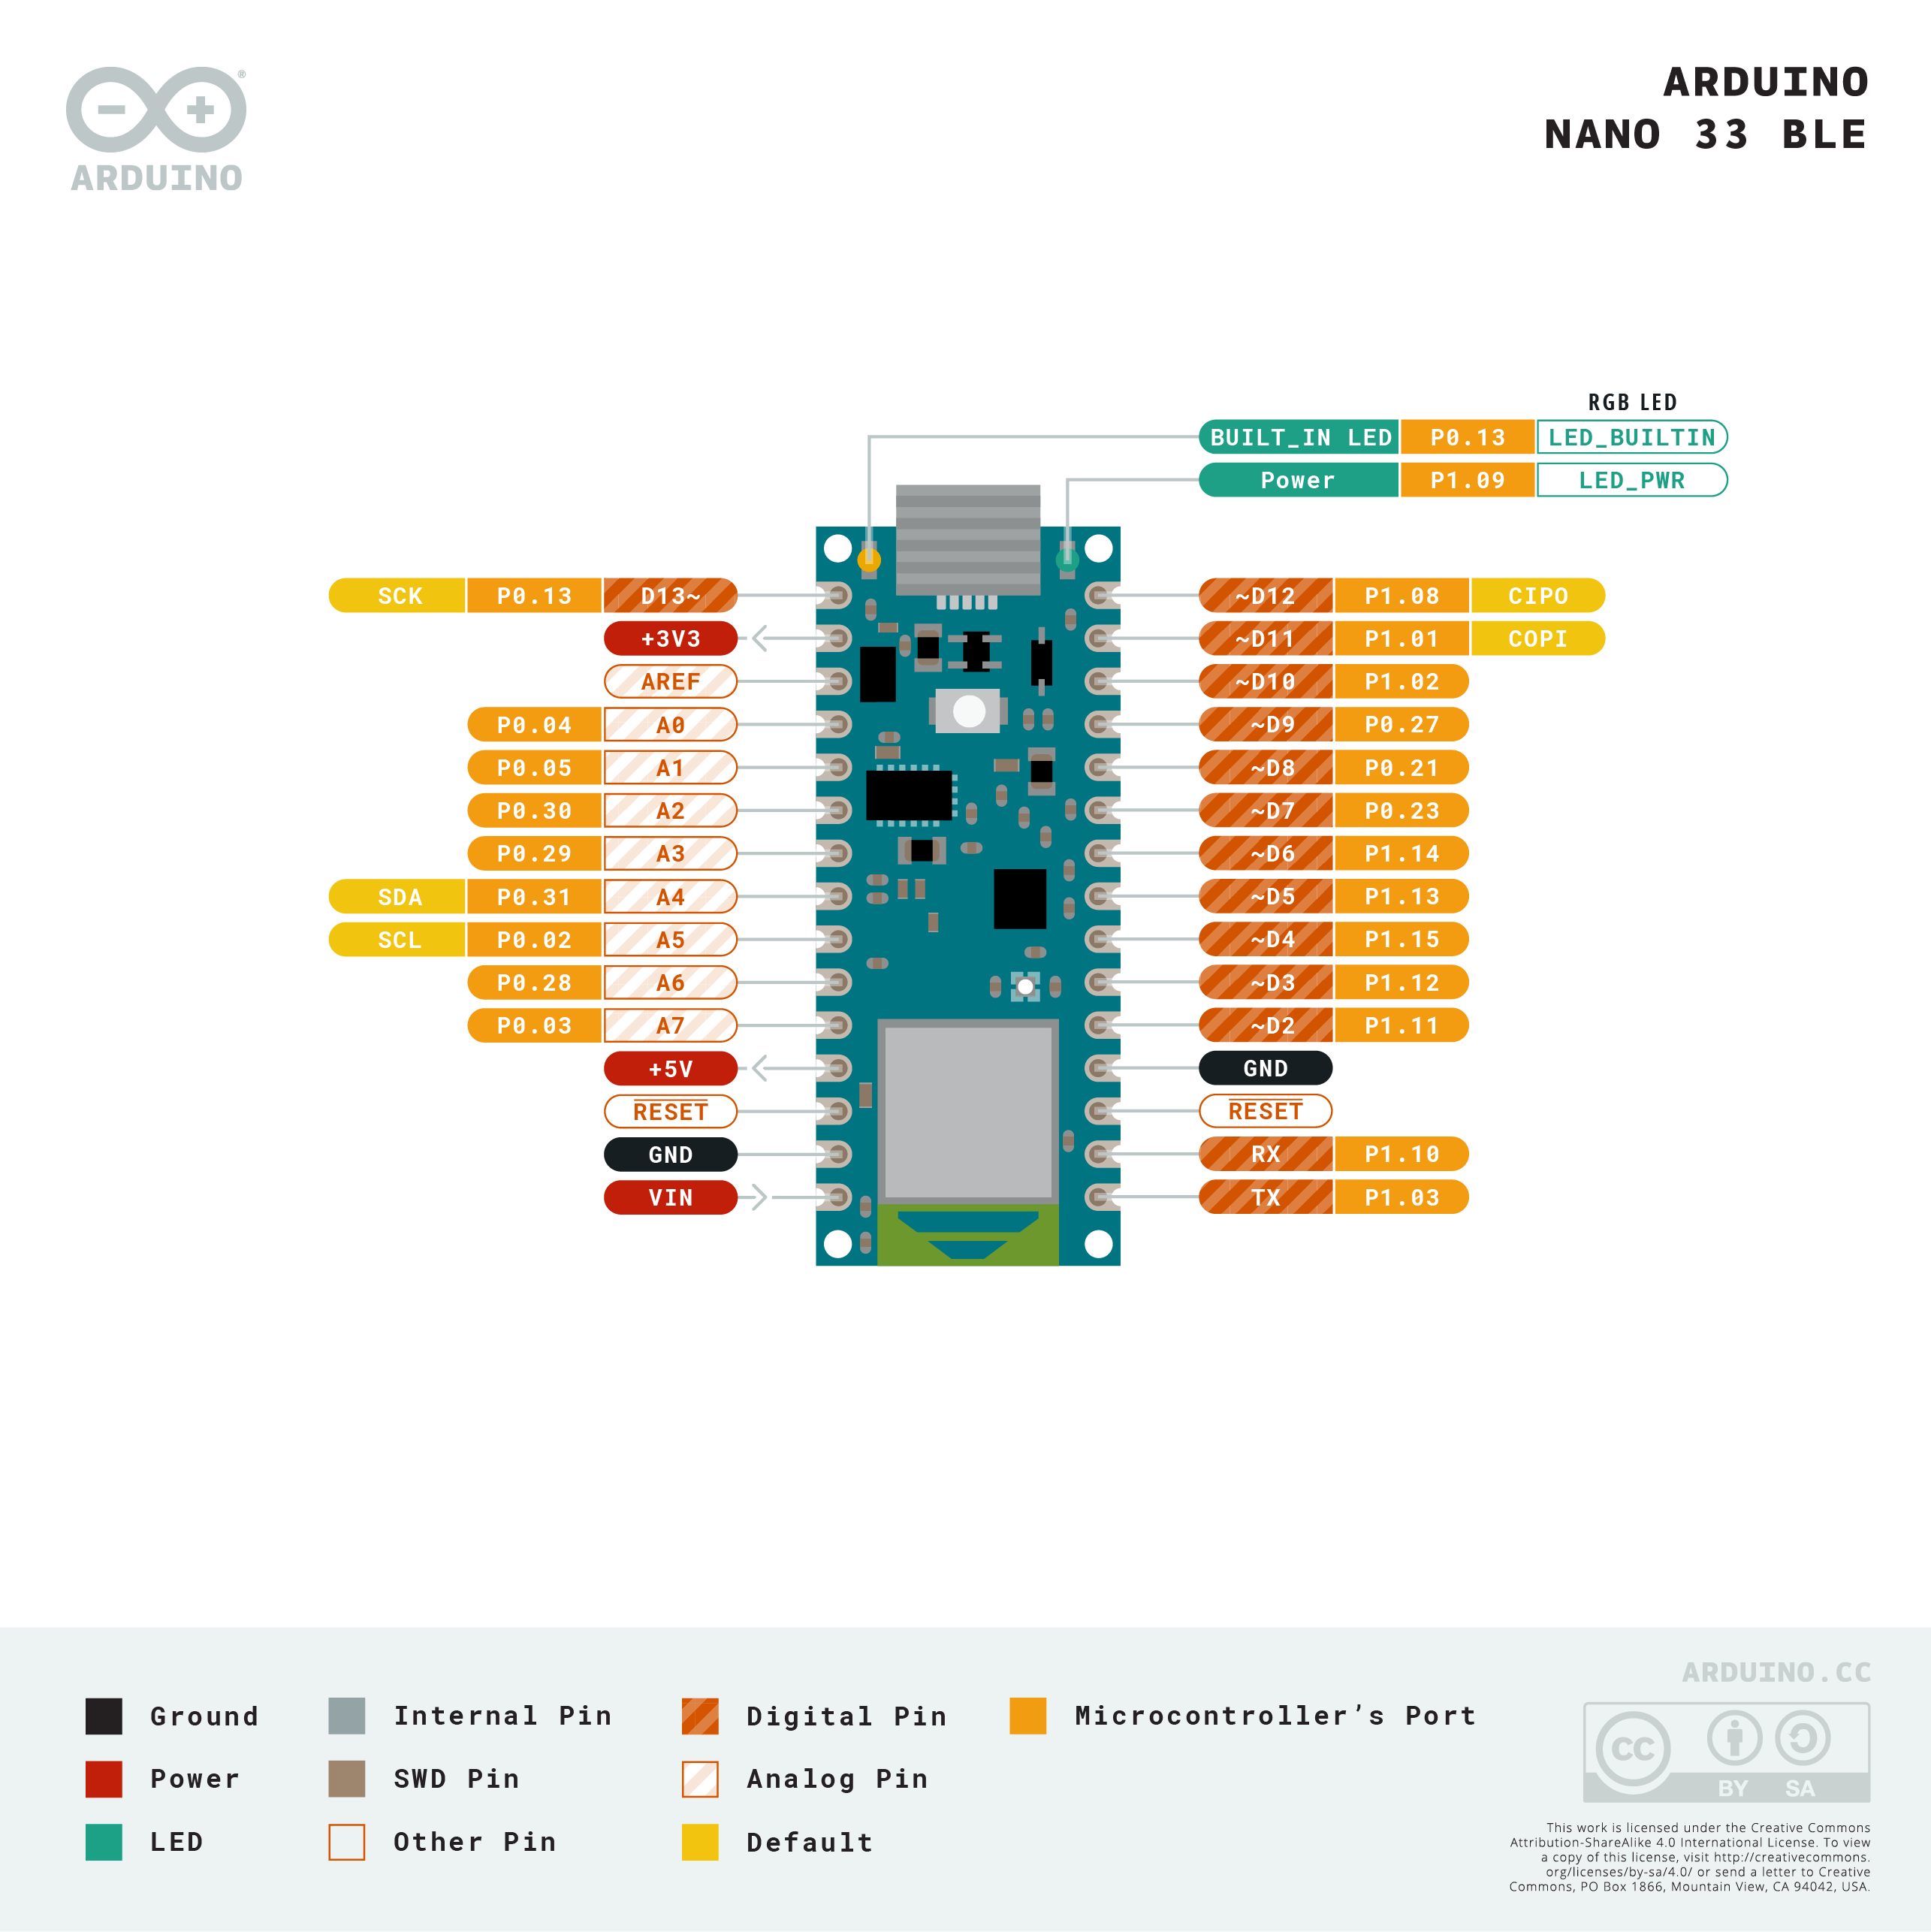
\includegraphics[width=\linewidth]{Images/pinout}
	%\caption{\textbf{Pinout}}\cite{Ard:2019}
%\end{figure}
%\newpage

%\section{Schematic connection diagram}
%\begin{figure}[h!]
%	\centering	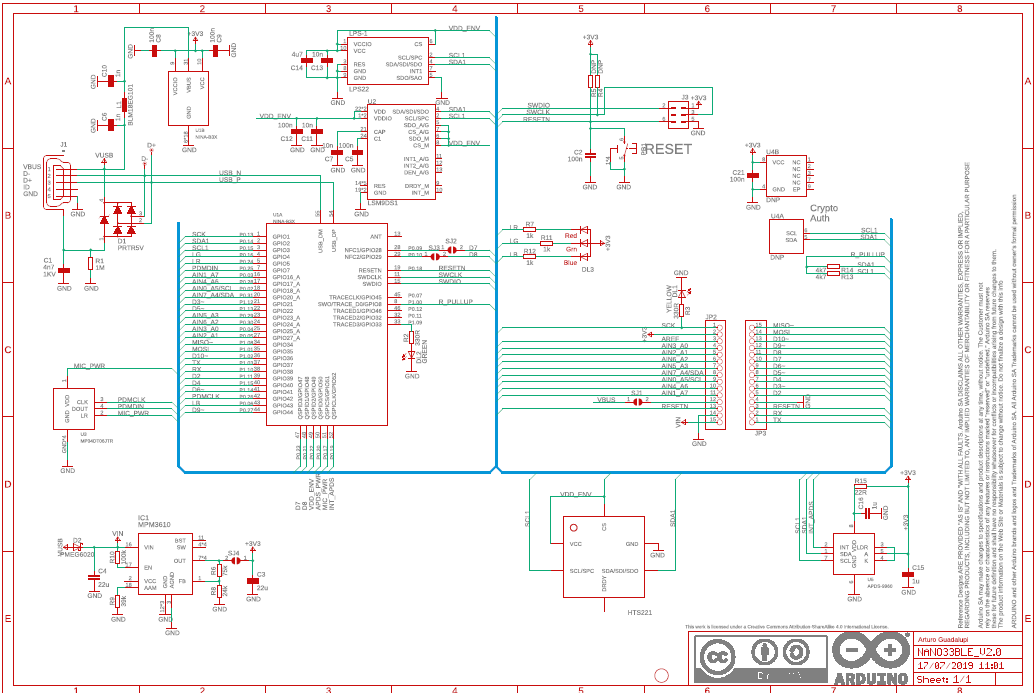
\includegraphics[width=\linewidth]{Images/schem}
%	\caption{\textbf{Schematic connection diagram}} \cite{Ard:2019}
%\end{figure}
